\documentclass{article}
\usepackage[T1]{fontenc}
\usepackage{lmodern}
\usepackage{graphicx}
\usepackage{amsmath,amssymb}
\usepackage[a4paper,margin=2cm]{geometry}
\usepackage[absolute,overlay]{textpos}
\setlength{\TPHorizModule}{1mm}
\setlength{\TPVertModule}{1mm}
\usepackage[indonesian]{babel}
\usepackage{hyperref}
\setlength{\emergencystretch}{2em}
% unit: Halaman 1

\begin{document}

% === Halaman 1 (llm) ===

\begin{center}
Bahan kuliah IF4020 Kriptografi

\vspace{10mm}
\Huge \textcolor{red}{04 - Kriptografi Klasik}
\large \textcolor{red}{(Bagian 2)}

\vspace{98.90mm}

\vspace{10mm}
\large Oleh: Rinaldi M

\vspace{20mm}
\textbf{Pogram Studi Teknik Informatika}\
\textbf{Sekolah Teknik Elektro dan Informatika}\
\textbf{Institut Teknologi Bandung}\
\textbf{2026}
\end{center}

% deskripsi: Ilustrasi mesin kriptografi klasik berupa silinder huruf yang dapat diputar untuk enkripsi.
% bbox normalisasi: [0.0470, 0.4330, 0.3030, 0.7660]
\begin{textblock*}{53.76mm}(9.87mm,128.60mm)
\noindent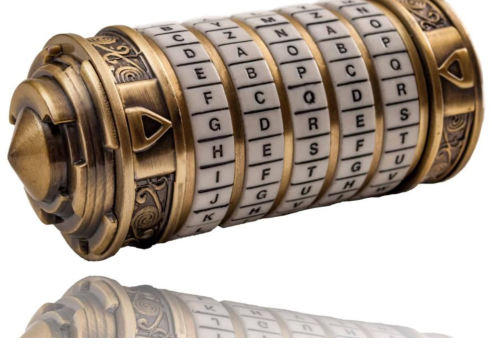
\includegraphics[width=53.76mm,height=98.90mm]{../../images/llm/page_001_img_01.png}%
\end{textblock*}

\end{document}
